\documentclass[lualatex, a4paper, ja=standard]{bxjsarticle}

\usepackage{luatexja}
\usepackage{graphicx}
\usepackage{amsmath, amssymb}
\usepackage{syntax}
\usepackage{fancyvrb}
\usepackage{url}
\usepackage{tikz}

% \setlength{\grammerparsep}{}
\setlength{\grammarindent}{16em}

\setpagelayout*{margin=20truemm}

\title{2022年度 コンパイラ実験 最終レポート}
\author{氏名:  \\ 学生番号: }

\begin{document}
\maketitle

\section{概要}
Flex,Bison を用いて,独自の言語を
maps で動作するアセンブリ言語に変換するコンパイラを作成する.

コンパイラのソースコードはGitHub
\footnote{\url{https://github.com/AAAR-Salmon/experiment-compiler/tree/compiler}}
にある.

\section{作成する言語の概要}

\subsection{文法}

この言語は次のような文法を持つ.
ただし,$\langle\mathit{identifier}\rangle$ は
正規表現 \verb/[a-zA-Z][a-zA-Z0-9]*/ に,
$\langle\mathit{number}\rangle$ は
正規表現 \verb/[0-9]+/ にマッチするトークンである.
また,\verb'#' から行末までをコメントとして扱う.

\begin{grammar}
<program> ::=
  <declarations> <statements>

<declarations> ::=
  <declaration-statement> <declarations> \alt
  <declaration-statement>

<declaration-statement> ::=
  `define' <identifier> `;' \alt
  `array' <identifier> `[' <number> `]' `;'

<statements> ::=
  <statement> <statements> \alt
  <statement>

<statement> ::=
  <assign-statement> \alt
  <loop-statement> \alt
  <branch-statement>

<assign-statement> ::=
  <reference> `=' <expression> `;'

<loop-statement> ::=
  `while' `(' <expression> `)' `{' <statements> `)'

<branch-statement> ::=
  `if' `(' <expression> `)' `{' <statements> `}' \alt
  `if' `(' <expression> `)' `{' <statements> `}' `else' `{' <statements> `}'

<reference> ::=
  <identifier> \alt
  <identifier> `[' <expression> `]'

<expression> ::=
  <expression> `and' <conditional-expression> \alt
  <expression> `or' <conditional-expression> \alt
  `not' <conditional-expression> \alt
  <conditional-expression>

<conditional-expression> ::=
  <additional-expression> `==' <additional-expression> \alt
  <additional-expression> `!=' <additional-expression> \alt
  <additional-expression> `<' <additional-expression> \alt
  <additional-expression> `<=' <additional-expression> \alt
  <additional-expression> `>' <additional-expression> \alt
  <additional-expression> `>=' <additional-expression> \alt
  <additional-expression>

<additional-expression> ::=
  <additional-expression> `+' <multiplicational-expression> \alt
  <additional-expression> `-' <multiplicational-expression> \alt
  <multiplicational-expression>

<multiplicational-expression> ::=
  <multiplicational-expression> `*' <primitive-expression> \alt
  <multiplicational-expression> `/' <primitive-expression> \alt
  <multiplicational-expression> `%' <primitive-expression> \alt
  <primitive-expression>

<primitive-expression> ::=
  <reference> \alt
  <number> \alt
  `(' <expression> `)'
\end{grammar}

\subsection{受理するプログラムの例}

以下に示すプログラムは必ずしも正常にコンパイルされるものではない.

\begin{Verbatim}[frame=lines, numbers=left]
define s;
define i;

s = 0;
i = 1; while (i <= 10) {
  s = s + i;
  i = i + 1;
}
\end{Verbatim}

\begin{Verbatim}[frame=lines, numbers=left]
array fib[20];
define i;

fib[0] = 0;
fib[1] = 1;
i = 2; while (i < 20) {
  fib[i] = fib[i-1] + fib[i-2];
}
\end{Verbatim}

\begin{Verbatim}[frame=lines, numbers=left]
define in1;
define in2;
define inc;
define outs;
define outc;

# set input here
in1 = 0;
in2 = 1;
inc = 1;

# outs = (in1 xor in2) xor inc
outs = (in1 and (not in2)) or ((not in1) and in2);
outs = (outs and (not inc)) or ((not outs) and inc);

outc = ((in1 and in2) or (in1 and inc)) or (in2 and inc);
\end{Verbatim}

\section{コード生成}

Bisonプログラムによって作成した抽象構文木(AST)を辿って生成する.

\subsection{メモリ領域}

0x00000000 から大きいアドレスがプログラムの初期化部領域,
0x00001000 から大きいアドレスがプログラムコード部領域,
0x10008000 から大きいアドレスがグローバル変数領域,
0x80000000 から\textbf{小さい}アドレスが計算用スタック領域である.

2領域がオーバーラップしたときの動作は保証されない.

\subsection{レジスタ}

このコンパイラにおける各レジスタの用途を,
表 \ref{tab:register} に示す.
示されていないレジスタは未使用である.

\begin{table}[b]
  \centering
  \caption{レジスタの用途}
  \label{tab:register}
  \begin{tabular}{|rl|l|} \hline
    レジスタ番号 & レジスタ名 & 用途 \\ \hline\hline
    0  & \$zero & 値 $0$ の参照 \\
    1  & \$at   & (アセンブラのために予約) \\
    2  & \$v0   & 式の評価値 \\
    3  & \$v1   & 式の評価値 \\
    4  & \$a0   & (関数のために予約) \\
    8  & \$t0   & 変数アドレスの計算用 \\
    26 & \$k0   & (OSのために予約) \\
    27 & \$k1   & (OSのために予約) \\
    28 & \$gp   & グローバル変数領域の先頭アドレス \\
    29 & \$sp   & 計算用スタックのトップアドレス \\
    30 & \$fp   & (関数のために予約) \\
    31 & \$ra   & (関数のために予約) \\ \hline
  \end{tabular}
\end{table}

\subsection{算術式のコード生成}

式のASTは,not演算子を除き,
図\ref{fig:ast-expression} のいずれかの形を取る.

続く小節ではそれぞれの場合のコード生成を説明する.
not演算子については取る式が1つであることを除き
二項演算と大きくは変わらないため省略する.

\begin{figure}[b]
  \centering
  \begin{tabular}{cccc}
    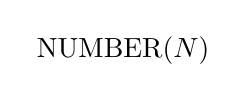
\begin{tikzpicture}
      \node{ NUMBER($N$) };
    \end{tikzpicture} &
    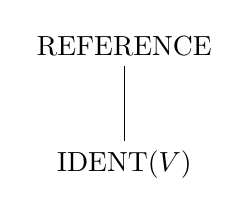
\begin{tikzpicture}
      \node{ REFERENCE }
        child { node { IDENT($V$) } };
    \end{tikzpicture} &
    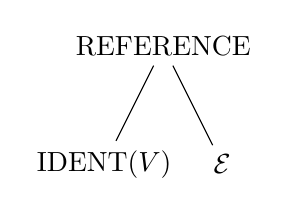
\begin{tikzpicture}
      \node{ REFERENCE }
        child { node { IDENT($V$) } }
        child { node { $\mathcal{E}$ } };
    \end{tikzpicture} &
    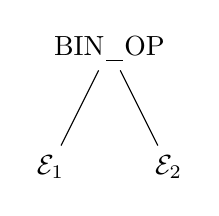
\begin{tikzpicture}
      \node{ BIN_OP }
        child { node { $\mathcal{E}_1$ } }
        child { node { $\mathcal{E}_2$ } };
    \end{tikzpicture} \\
    定数 & 変数 & 配列要素 & 二項演算
  \end{tabular}
  \caption{式のAST ($\mathcal{E}, \mathcal{E}_1, \mathcal{E}_2$ は
    式のAST)}
  \label{fig:ast-expression}
\end{figure}

\subsubsection{定数}

ASTから値 $N$ を取得し,
疑似命令 \verb|li  $v0,| $N$ に対応するコードを生成する.

\subsubsection{変数}

\begin{enumerate}
  \item ASTから変数名 $V$ を取得し,
  記号表から対応するアドレスオフセット $d$ を計算する.
  \item 疑似命令 \verb|li  $t0,| $d$ に対応するコードを生成する.
  \item コード \verb|addu  $t0, $gp, $t0| を生成する.
  \item コード \verb|addu  $v0, 0($t0)| を生成する.
\end{enumerate}

\subsubsection{配列要素}

\begin{enumerate}
  \item 算術式 $\mathcal{E}$ のコード生成をする
  ($\mathcal{E}$ を評価した値が \verb|$v0| に格納されている).
  \item コード \verb|sll  $v0, $v0, 2| を生成する.
  \item ASTから変数名 $V$ を取得し,
  記号表から対応するアドレスオフセット $d$ を計算する.
  \item 疑似命令 \verb|li  $t0,| $d$ に対応するコードを生成する.
  \item コード \verb|addu  $t0, $t0, $v0| を生成する.
  \item コード \verb|addu  $t0, $gp, $t0| を生成する.
  \item コード \verb|addu  $v0, 0($t0)| を生成する.
\end{enumerate}

\subsubsection{二項演算}

\begin{enumerate}
  \item 算術式 $\mathcal{E}_1$ のコード生成をする
  ($\mathcal{E}_1$ を評価した値が \verb|$v0| に格納されている).
  \item \verb|$v0| をスタックにプッシュするコードを生成する.
  \item 算術式 $\mathcal{E}_2$ のコード生成をする
  ($\mathcal{E}_2$ を評価した値が \verb|$v0| に格納されている).
  \item スタックから値をポップし,\verb|$v1| に格納するコードを生成する.
  \item (この段階で第1オペランドは \verb|$v1| に,
  第2オペランドは \verb|$v0| に格納されている.)
  \item 二項演算子(中置)を $\circ$ としたとき,
  「\verb|$v1| $\circ$ \verb|$v0| を \verb|$v0| に格納する」
  に対応するコードを生成する.
\end{enumerate}

\end{document}
